\begin{figure}[h!]
\centering
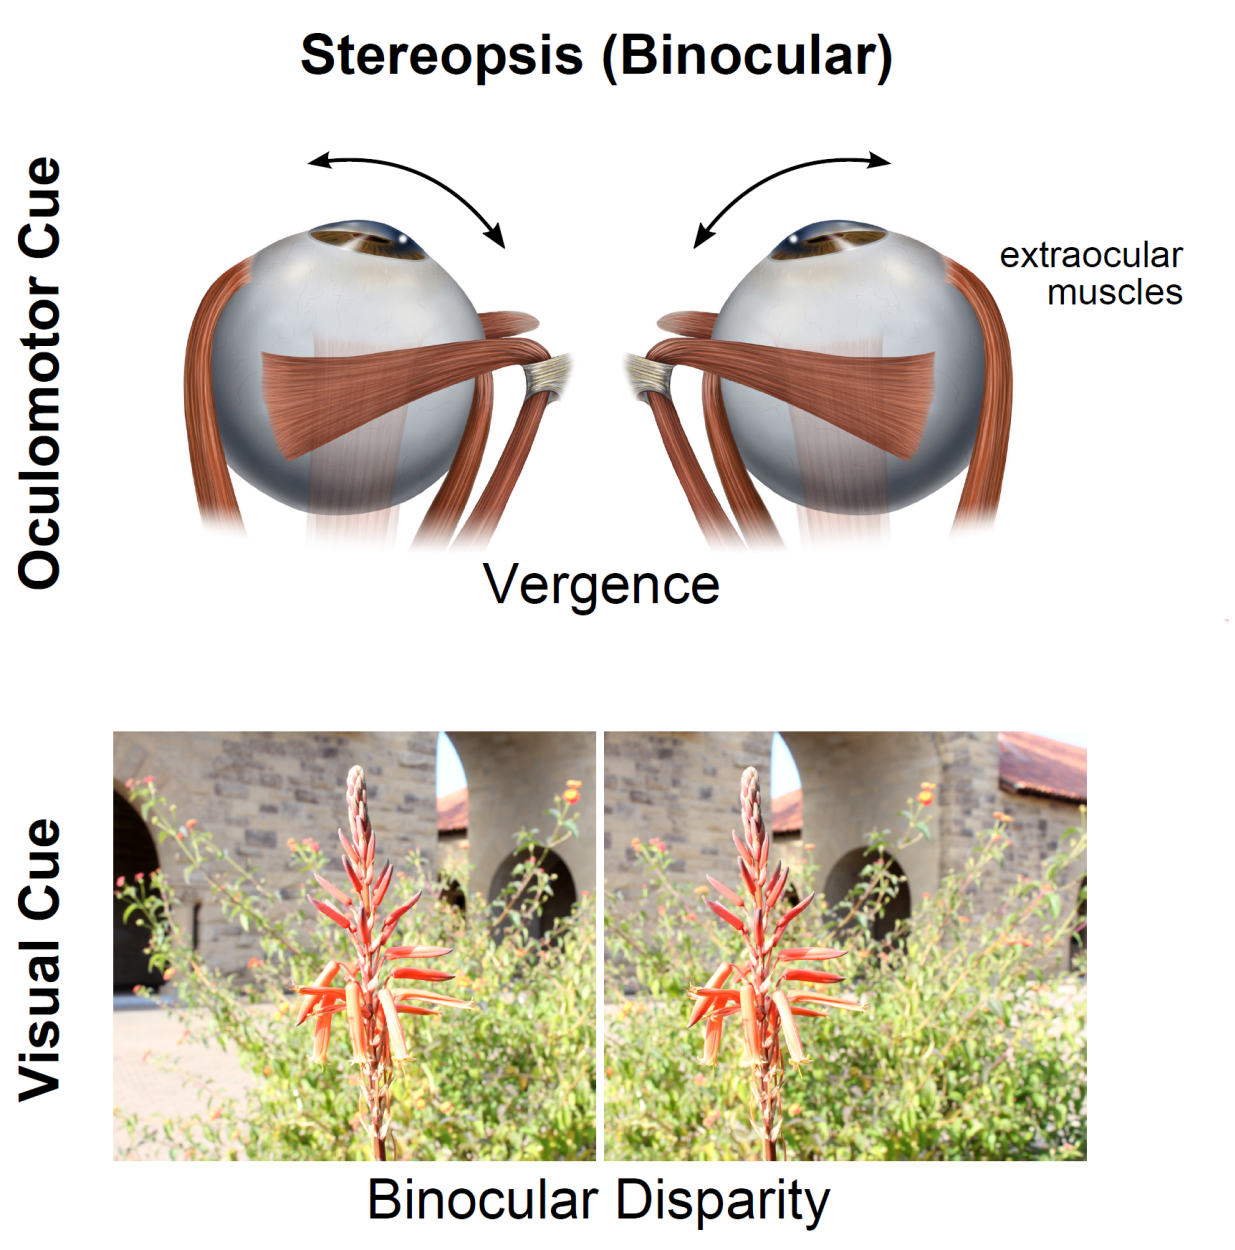
\includegraphics[width=0.59\columnwidth]{images/other/binocular_depth_cues}
\caption[Binocular depth cues]{We perceive depth from these binocular cues (1) \emph{convergence:} our eyes rotate to form the image of the object of attention at our retina, and (2) \emph{disparity:} the images formed in our two eyes are slightly different. Image source: Adapted from \cite{Konrad2017Accommodation}}
\label{fig:cones_and_rods_distribution}
\end{figure}

